\subsection{Li-Chao Tree}

Reference : \href{https://robert1003.github.io/2020/02/06/li-chao-segment-tree.html}{A Simple Introduction to Li-Chao Segment Tree}

Li-Chao Tree is an upgrade of Convex Hull Trick. Instead of monotone slope in CHT, it can handle both arbitrary slope and query.

Given 2 types of queries, add a line to multiset $S$, find the maximum value at some point $x$. It can handle both of the query with $\mathcal{O}(\log{X})$ where $X$ is the maximum value of type-2 query. We will use a Segment Tree to store the best line for some range $[l, r]$. We can even do lazy propagation, sparse (dynamic node creation), or persistent with it.

We will use each node of the segment tree as a Line.

\begin{lstlisting}
struct Line {
    ll m = 0, c = LLONG_MIN; // c = LLONG_MAX for min Li-Chao Tree
    ll operator()(ll x) { return m * x + c; }
} seg[4*mxX];
\end{lstlisting}

\subsubsection{Insertion}

For conveinence, we assume $m_\text{new} < m_\text{old}$ (if not, then swap the lines). We will consider 2 cases.

\begin{figure}[h]
    \centering
    \begin{minipage}{0.48\textwidth}
        \centering
        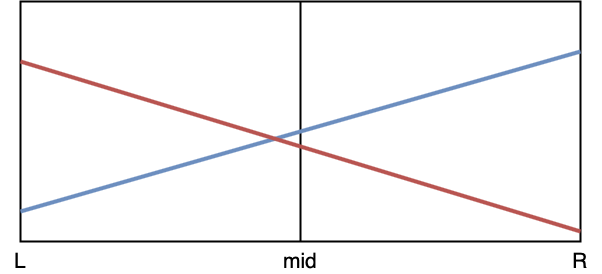
\includegraphics[width=\textwidth]{assets/lichao_1.png}
        \caption*{Case 1}
    \end{minipage}
    \hfill
    \begin{minipage}{0.48\textwidth}
        \centering
        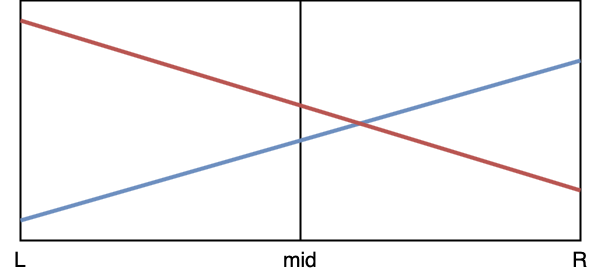
\includegraphics[width=\textwidth]{assets/lichao_2.png}
        \caption*{Case 2}
    \end{minipage}
\end{figure}

Case 1 -- $f_\text{new}(\text{mid}) < f_\text{old}(\text{mid})$: The old line is better for range $[l, r]$, except some range in the left side, so we recursively insert the new line to the left.

Case 2 -- $f_\text{new}(\text{mid}) > f_\text{old}(\text{mid})$: The new line is better for range $[l, r]$, except some range in the right side, so we recursively insert the old line to the right.

\begin{lstlisting}
void ins(int l, int r, Line x, int u) {
    if (l == r) {
        if (seg[u](l) < x(l)) seg[u] = x;
        return;
    }
    int m = l + (r-l)/2;
    if (x.m > seg[u].m) swap(x, seg[u]);
    if (x(m) < seg[u](m)) ins(l, m, x, u<<1);
    else swap(x, seg[u]), ins(m+1, r, x, u<<1|1);
}
\end{lstlisting}

\subsubsection{Query}

We just query for point $x$ normally, but we have to get the maximum with the current line too.

\begin{lstlisting}
ll qr(int l, int r, int x, int u) {
    if (l == r) return seg[u](x);
    else {
        int m = l + (r-l)/2;
        if (m >= x) return max(seg[u](x), qr(l, m, x, u<<1));
        else return max(seg[u](x), qr(m+1, r, x, u<<1|1));
    }
}
\end{lstlisting}

\break